\documentclass[]{article}
\usepackage{amsmath}
\usepackage{siunitx}
\usepackage{graphicx}
\usepackage{float}
% Title Page
%\title{Documentation summary}

\begin{document}
\tableofcontents
\newpage
\section{Torque and Pitch Angle Control for Variable Speed Wind Turbines in All Operating Regimes \cite{5874598}, pag. 3-4}
A multivariate controller acts both on rotor speed and electrical power. 
\begin{itemize}
	\item Below rated: Maximum power extraction; variable rotor speed and constant pitch angle; torque controller allows to work following the MPPA
	\item Above rated: pitch angle controlled to maintain constant power while the torque controller regulates the rotor speed to keep the constant nominal speed. 
\end{itemize}
Reference torque produced by an estimator.\\
In this work the torque controls the rotational speed and the pitch control the power\\
Optimal tip speed ratio and rated wind speed are computed beforehand. \\
The turbine works in three regions: region 1 is the one below rated wind speed where the turbine stars-up; region 2 is in between cut in and rated power (here pitch is constant and the rotor speed is kept constant by changing the torque control) here small changes in the pitch angle about the optimal can be done in order to reduce the dynamic load; region 3 is above the rated wind speed where we want to limit the output power to the rated one. Make the transition smooth between the regions. \\
\begin{gather}
	P = \frac{\pi \rho cp R^2 v^3}{2}\\
	T = \frac{P}{\omega}\\
	J \frac{d \omega}{d t} = T_{t} - T_{generator} -K_t\omega_t
	\label{eq:dynamic_rotor_gen}
\end{gather}
with J the total inertia, $K_t$ is the total damping.\\
Torque controller implemented estimating the the aerodynamic torque with an estimator. Pitch controller implementing the angle as function of the error between the actual power and the nominal one.\\
In the work a permanent magnets synchronous generator is used. The d-q current components are controlled via a PI controller. \\
Torque estimation is quite good and so the speed tracking. The steady state tracking error is removed by the integral action on the torque estimator.\\
The reference rotational speed is carried out from the measurements on the wind speed, however there are other methods to define the reference speed without wind speed measurements to avoid inaccuracy of the measurements and its relation to the wins speed as this is perceived by the wind turbine.
\newpage
\section{Control of Wind Turbines \cite{5160195}}
Usually the rotor drives the generator via a a steps up gearbox but direct drive configurations are becoming more popular in order to eliminate possible source of failures. \\
Variable speed wind turbines require electrical power processing in order to fulfil the grid requirements. They are also able to reduce loads because possible gusts are absorbed as rotational speed increase rather than as component bending.\\
Three blades turbines experience more symmetrical loading than two bladed turbine.  
\subsection{Wind speed variation}
Wind turbines have difference levels of control: supervisory, operational, and subsystem. Supervisory determines when the turbine starts and stops in response to changes in the wind speed and also monitors the health of the turbine. The operational determine how the turbine achieves its control objective in regions 2 and 3. The subsystems are responsible for the generator, power electronics yaw drive, pitch drive and other actuators.\\
The wind speed may or may not been assumed constant across the rotor swept area, in time and space. These variations may be considered as disturbances for control design. The assumption of constant wind speed may lead to poor results especially for large size turbine. \\
In order to capture the wind speed variations along the blade, then hundred of sensors would been necessary to characterize the wind distribution along the blade. The most important parameters to characterize the wind are: spatial and temporal average, frequency distribution of wind speed, temporal and spatial variation, prevailing wind direction. There are different time scales: long time scales are used for determining whether a location is suitable for siting a wind turbine; daily scale affects mainly the direction and it is due to different heating of the surface; hourly is used to plan the mixing of different resources in the portfolio; short term prediction is used to mitigate structural loading during gusts and turbulence. \\
\subsection{Sensors}
The rotor speed measurement is used as feedback for basic control (ie speed and power) in region 2 and 3. It can be measured either before or after the gearbox.\\ Anemometer is used to determine whether the wind speed is sufficient for starting the turbine operation. The wind measurement is distorted by the rotor-wind interaction, so the measurement is not always reliable. \\
Measurements must be reliable, and fault identification can be used to identify faulty sensors. 
\subsection{Actuators} 
Yaw motor: aligns the nacelle with the wind; turbine cannot be yawed at high rates due to gyroscopic effects (a typical rate is 1 \si{\degree}/s). The control ofthe yaw provides less benefit rather than the others.\\
Generator: can be controlled to follow a desired torque and so determines how much torque is extracted from the turbine. The generator torque can be used to accelerate and decelerate the rotor. \\
Bade-pitch motor: is restricted to approximately 5 \si{\degree \per \second} during the shut down of the turbine in region 1, while it can be around 8 \si{\degree \per \second} in 5 MW turbines. The blades can be controlled to pitch collectively or independently. 
\subsection{Control loops}
In region 2 the controller tries to maximize the power coefficient (ie optimal pitch angle), and so varying the pitch according to the incoming wind speed. \\
In region 3, the control is done by a pitch control loop, limiting the power and the speed in order to not exceed the electrical and mechanical load. \\
Controllers and effects are frequently coupled, especially in complex turbines. 
\subsubsection{Generator torque control}
\subsubsection{Pitch control}
Pitch control in region 3 is done with a PID controller, but usually only just a PI is used. \\
The basic controller is the SISO independent pitch controller, while if also other measurements are taken into account (ie strain gauge measuring the blade bending moment) then a MIMO individual pitch controller can be designed. 
\subsubsection{Switching regime}
Alongside with region 2 and 3 there is frequently even a third region, called region 2.5 which is used to facilitate the switch between the other two. This regime should be carefully considered because the linear connection often used may no result in smooth operations. \\
Particularly important is also the control during the emergency switch off of the turbine, and also the use of the emergency break should be carefully considered. \\ \\
Further advanced control strategies are presented in the publication.
\subsection{Control of wind farm}
There are different configurations in which the turbine can be placed in the farm. \\
The controller may wants to set active and reactive power supplied to the grid.\\
Due to the modification of the wind flow, it is not true that if all the turbines in the farm extract the maximum power than also the farm extracts the maximum available. This happens because the first turbine slow down the wind a lot and so the ones in the wake may experience a slower wind speed and so they are able to extract less power.\\
An important decision parameter is the spacing of the turbine both in the direction of the wind and in the perpendicular one. 
\newpage
\section{Description of the DTU 10 MW Reference Wind Turbine}
\subsection{Drivetrain properties}
The DTU 10 MW has a medium speed gearbox design. This is a compromise between direct drive generators (where the rare hearts are expansive) and the high speed gearboxes (with high risks of failure).\\
The rated rotor speed is 9.6 [rpm] = 1.0048 [rad/s] and a rated generator speed of 480 [rpm] with a gearbox ratio of 50:1. The gearbox is assumed a double-stage gearbox with no friction losses.  \\
The TSR used below the rated wind speed is 7.5.
\newpage
\section{10-MW Direct-Drive PMSG-Based Wind Energy Conversion System Model}
This work presents a model for a 10 mw direct-drive wind energy conversion system, considering also wind shear and tower shadow effects. The control is based on the theoretical maximum power curve.\\
\subsection{Introduction}
Tower shadows and wind shear are not always considered in the modelling of WT, as long as the working operations in region different from the MPPT, but here they do so. The investigate turbine is direct drive.
\subsection{System Description}
\textbf{Wind Turbine Modeling}\\
The aerodynamic torque is computed by
\begin{equation}
	T_{aero} = \rho \pi R^3 V_w \frac{C_p(\lambda, \beta)}{\lambda}\left[\frac{V_w}{2} + V_w^{WS} + V_w^{TS}\right]
\end{equation}
Where $V_w$ is the nominal windspeed, $V_w^{WS}$ is the windspeed taking into account the wind shear, and $V_w^{TS}$ is the one taking into account the tower effect. $V_w^{WS}$ and $V_w^{TS}$, which are angle depending terms, are considered because otherwise the torque equation does not represent well the power fluctuations occurring in high power WTs. Their effect may produce an oscillations fo the electric quantities in the range 0.5-2 Hz. Models for $V_w^{WS}$ and $V_w^{TS}$ are reported in the article. \\
\textbf{PMSG}\\
The chosen genrator is a isotropy PMSG (ie permanent magnets are mounted on the surface of the rotor). It is modeled in the dq synchronous reference frame, so the d and q axis are equal to the ones in the \textit{Azionamenti elettrici} notes. The generator torque may be modelled as by the quadrature current component. \\
The rotor-generator dynamic are controlled by Eq. \ref{eq:dynamic_rotor_gen} in which J is the equivalent rotational inertia, considering the rotor and drivetrain dynamic:
\begin{equation}
	J = \frac{J_{turbine}}{n_{gearbox}^2} + J_{gearbox}
\end{equation}
\subsection{Proposed control system}
The control has to: process the maximum amount of energy at different wind speed, increase efficiency, increase useful life of the WT, decrease structural mechanical effort, reduce energy production downtime, provide optimum dynamic performances, ensure system stability. The control is based on the typical theoretical power curve, featuring 5 operating regions.\\
Region 1: the low wind speed does not provide enough torque to make the rotor turn and furthermore this low speed rotation may force a low frequency vibration of the tower. For those reasons, the generator is kept braked. Furthermore the blades are kept pitched at 90 \si{\degree}.\\
Region 2: MPPT algorithm must be applied to extract the maximum power provided by the wind, and the pitch angle is kept at the value of maximum aerodynamic efficiency (usually 0\si{\degree} ). In this work the control is done with a method called Optimal Torque Control. Even though it has a slower dynamic response to variations in wind speed, it provides smoother transitions wrt to other methods. This reduces the mechanical stress on the components of the wind system. The OTC uses a rotational speed sensor and $\omega_m$ is used to compute the mechanical torque reference, assuming that the turbine works with the most convenient Cp and $\lambda$: 
\begin{equation}
	T_{w}^*=0.5 \rho \pi R^5 \frac{C_{p,max}}{\lambda_{opt}}\omega_m^2
\end{equation} 
In the steady state and neglecting the losses, the electromagnetic torque is approximately the mechanical torque, rescaled by the gearbox transformation ratio. The OTC method is used as an electromagnetic torque reference:
\begin{equation}
	T_e^* = T_{w}^*/n_{gearbox}=0.5 \rho \pi R^5 \frac{C_{p,max}}{\lambda_{opt}^3n_{gearbox}^3}\omega_{gearbox}^2
\end{equation}
Region 3: it is a transition region between 2 and 4. In this region the rotational speed is kept constant at its nominal value and the pitch is 0 \si{\degree}. This implies that the maximum power is no longer a priority as opposed to operation within region 2. The control variable is the nominal rotational speed of the generator. A PI controller can be designed.  This reagion of operation is not always present.\\
Region 4: is the power limiting one, and the control is done changing the pitch angle of the blades. The actuation mechanism consists of a servo motor, modeled as a first order function. The output of the servomotor is limited within 0-90 \si{\degree} and the pitch rate is limited between $\pm$ 3 \si{\degree \per \second}.\\
Region 5: It is the region where the WT is shut down because the windspeed is above the maximum allowed one.
\subsection{PMSG current control}
The input parameters are torque and/or angular speed and/or voltage of the DC bus of the machine side converter. In this work the control is applied using the Field Oriented Control FOC, aimed to keep the direct axis (d-axis) constantly aligned with the flux vector permanent magnet. The referent current $i_{d,s}^*$ must be kept at zero, while the reference for the $i_{q,s}$ is determined by the speed or power control system.\\
The FOC control technique is composed by two independent current control loops whose $i_{q,s}^*$ is :
\begin{equation}
	i_{q,s}^* = \frac{T_e^*}{1.5p \lambda_m}
\end{equation}

\newpage
\section{Offshore Wind Energy Technology \cite{Olimpo_Anaya‐Lara}}
\subsection{Modeling and analysis if drivetrains in offshore wind turbines}
Wind turbine drivetrains are made of components that have been used successfully in many other industries, the failure rates of drivetrains has been a concerned in the wind industry. The problem is not the failure rate but the long downtime needed to repair or replace a part of the drivetrain. The reliability of the gearbox is an important feature.\\
Gearboxes are primary used to increase the rotational speed to facilitate the use of high speed generators. A typical high speed gearbox has three stages of planetary gears and parallel gears. Direct drive WT are the most common gearless technologies. Rotor and generator speed is the same. In that case the generator has to have a large number of poles. Advantages are low number of mechanical components while disadvantages are the weight and material cost. Some researchers highlighted that removing the gearbox does not necessary increase the reliability. \\
Medium speed gearboxes (ratio about 1/10) are in between high speed and direct drive.  \\
Adding a gearbox in the drivetrain amplifies the inertia of the transmission, making it less sensitive to the torque variation and limiting the fatigue life of the components. \\
Planetary gearboxes are widely employed due to their compact design, limited weight and low cost. The disadvantage is an increased complexity and difficulties of access, and they are more sensitive to the manufacturing errors.\\
According some researchers the less reliable subassemblies are: pitch mechanism, power electronic converter, yaw system, control system, generator, gearbox.
\subsection{Offshore wind turbine controls}
The flexibility of the blade must be taken into account in the tuning of the control system. Furthermore the presence of the submerged structure and the corresponding wave-tower interaction must be taken into account.
\subsubsection{5.1}
The primary objective of the wind turbine controller is to keep the rotor speed of the
wind turbine within limits, as it generates power. Secondary objectives include reducing
aerodynamic loads and structural vibrations, and providing ancillary services to the
electric grid. A supervisory level of control detects and handles operator commands,
faults, and extreme events, and initiates startup and shutdown sequences, as appropriate.\\
The turbine rating is defined as the electric power, bu the aerodynamic one is slightly higher.\\
The rotor speed has two boundaries: an upper and a lower one. The upper limits the load on the blades while the lower is necessary to avoid the excitation of the lowest tower resonant frequencies. At the start up (ie between 4 and 7 m/s) the blade pitch is set to maximize the aerodynamic power.\\
The turbine gas to respond to 3 loads due to wind and waves: the steady state ones (associated with the power extraction and gravity cycles in rotating components), the fluctuating loads at frequencies not near resonance, and the third is the resonance response.\\ 
Active and reactive power are almost independently controllable. It is meaningless to command a sustained active power higher than that which can be extracted from the wind. Operation in short‐term transients above the available aerodynamic power is possible by drawing down the kinetic energy of the spinning rotor. This subsequently requires a recovery period of reduced power generation, in order to re-accelerate the rotor.\\
The turbine has to deviate from the normal operation, such as during start up and shutdown sequences.\\
The power output can be regulated actively or passively. The latter us done with aerodynamic stall while the former with blades pitching or adjusting the torque. The active control helps to damp structural vibrations and provides grid support functions. The nacelle yaw is also actively regulated but it has a slower dynamic compared to the others.
\subsubsection{5.2}
SISO control: The simplest controller for a pitch‐regulated, variable speed wind turbine consists of a blook‐up table for the generator torque, as a function of rotor speed, and a PI controller for collective blade pitch, which becomes active when the rotor speed hits its rated value. The sole sensor input required for normal operation is a measurement of the shaft speed. The gain of the PI controller should be scheduled as a function of the wind speed. The results is not robust in the sense that it may give a significantly different performance if implemented on a model other than that with which it was tuned. Additional single‐input, single‐output pathways are added in order to fulfil specific secondary objectives. Each objective is assigned either to the generator torque or the blade pitch action; thus, tower fore–aft damping is provided by blade pitch, while side‐to‐side damping is provided by generator torque. \\ 
Advanced controls: The estimated wind speed may be used to improve the controller. \\
Multiple‐input, multiple‐output control systems are typically formulated in statespace and based around a model of the plant that is embedded within the controller. A distinction is made between linear parameter‐varying models – those which are formulated using linear theory and scheduled on the basis of one or more slowly‐varying parameters – and truly nonlinear models. It is possible to design control algorithms that adapt themselves online, during operation, in order to incrementally improve performance towards some optimum. Such adaptive, evolutionary or intelligent control algorithms do not necessarily require an embedded model.\\
A basic control strategy assigns each input control function to either the blade pitch or the generator torque. One SISO path is designed for each function. It is possible to design almost independent path, with only a small amount of coupling between them, but best performances are not obtainable in such a way.  \\
REGION 1: power command is set as cubic function if the measured speed. Alternatively, a speed tracking mode is active when operating at the minimum rotor speed. Here a PI controller drives the speed error to zero. Only one of these two pathways is active at a given time. The transition between modes may be scheduled as a function of the estimated windspeed, or blade pitch angle.\\
REGION 2: The basic rotor speed control function is the path that leads from the rotor speed error $\Omega - \Omega_{ref}$ through to the collective blade pitch command $\beta$. The operations at minimum speed are controlled in a specific way, also using an estimation of the wind speed. \\
Individual pitch is used to take into account the wind sheer. 
\subsubsection{5.3}
Pitch actuators: three strategies may be used to model the pitching dynamics. The simplest is to neglect the pitch actuator, and to assign the blade pitch angle directly from the control command. This simplification may be useful for some kind of controllers. The second modelling strategy is to represent the pitch actuator with a low order transfer function, and a second order one represents the most important effects. In the book there are also some indications of he parameters to be used in the transfer function. There are bounds on the maximum pitching rate. Since the dynamic of the pitching blade is complicated, then it should be implemented in combination with a full aeroelastic model of the rotating blade. The model proposed in the book considers a spring and a damper for connecting the pitching actuation mechanism with the blade.

\newpage
\section{Comparison of the obtained cP with the reference ones}
The obtained cP and cT are compared with the ones retrieved from the literature. In particular the value of the cP and cT values in the two operating regimes of the turbine are read directly from the \cite{DTU_Wind_Energy_Report-I-0092}, while the parametric relation between cP, $\lambda$ and $\theta$ are read from \cite{Variable-speed_Variable-pitch_control_for_a_wind_t}. The plots done by me are produced by the file cp\_comparison. 
\begin{figure}[H]
	\centering
	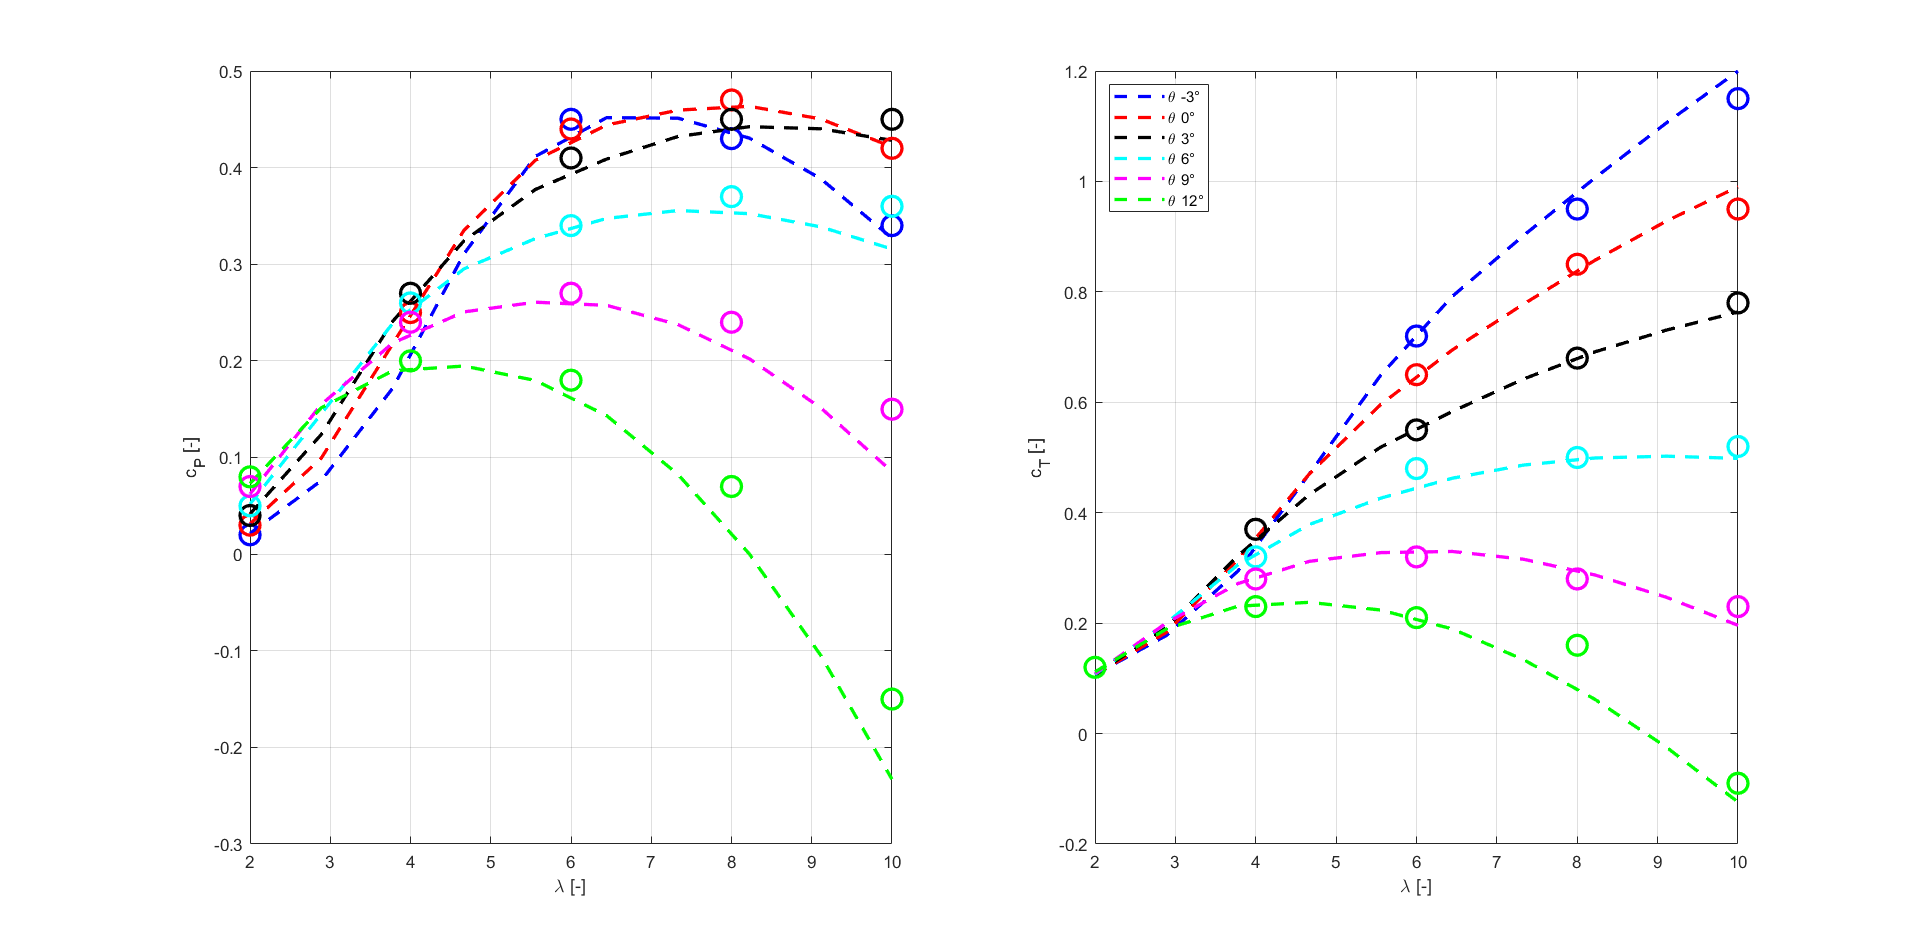
\includegraphics[width=0.7\linewidth]{images/cp_parametric_comp.png}
	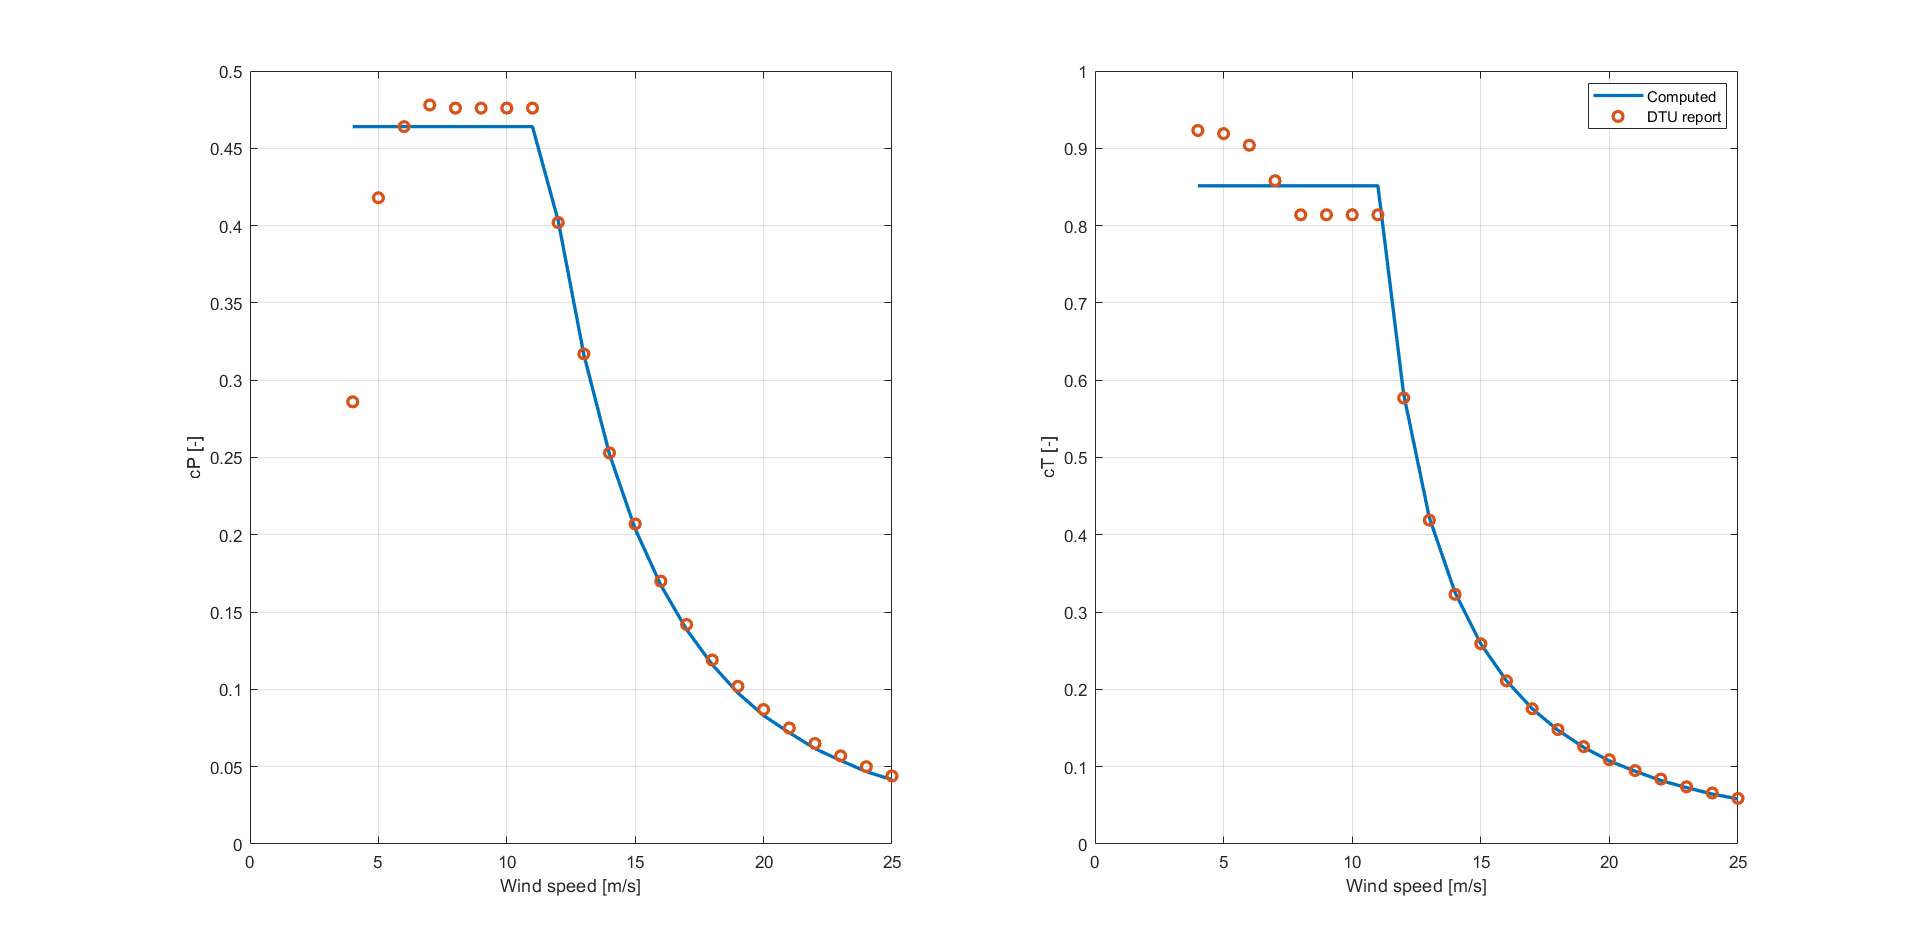
\includegraphics[width=0.7\linewidth]{images/cp_DTU10MW_comp.png}
	\caption{}
	\label{fig:cpparametriccomp}
\end{figure}

\newpage
\section{Reduce Order model for control applications in offshore wind turbine  \cite{SMILDEN2016386}}
The wind turbine control system contribute to the dynamic behaviour of the structure through its influence on aerodynamic damping, and ability to affect load variations caused by turbulence and the rotational motion of the rotor. The control system can therefore be used to lower the fatigue contributions from both wind and wave loads, allowing for a more marginally designed structure. \\ 
The model developed in this work includes a polynomial based approximation of the rotor aerodynamic:
\begin{gather}
	T_G = \frac{1}{2}\rho\pi R^3 C_Q(\theta, \lambda) V_0^2\\
	C_Q(\theta, \lambda) = a_{00} + a_{01}\lambda +a_{01}\lambda^2 + a_{10}\theta + a_{20}\theta^2 + a_{11}\theta\lambda + a_{21}\theta^2\lambda + a_{12}\theta\lambda^2 \\
\end{gather} 
The coefficients are obtained by curve fitting.\\ 
The drivetrain dynamic may include also the presence of a shaft with a finite stiffness and damping coefficients.\\ 
The switching between the two classical control regions is based on the power curve as it exceeds the rated on. Below rated the control low is based on the equation 
\begin{equation}
	T_G = \frac{1}{2 \lambda_{opt}^3}\rho \pi R^5 _{p,opt}\omega_G^2 = K_{opt}\omega_G^2
\end{equation}
Above rated the blades are pitched ti feather. The controller is a PI one, as shown in the publication and on the notes (pag. 17-18).
\newpage
\section{Basic DTU Wind Energy controller \cite{DTU_Wind_Energy_E_0028}}
The torque reference Qref,k at the current step k is computed based on a second order low-pass filtered LSS generator speed as $K\bar{\Omega_k}$. \\
The torque reference will then be given by the PID controller based on the speed error eQ,k = $\bar{\Omega_k} - \Omega_{set,k}$, where the set point is the minimum, or rated speed.\\
Because the rotor speed is bounded, the power loss can often be minimized be performing some adjustment of the minimum pitch. A first order lowpass filtered wind speed measured at hub height Vk is used as parameter for varying the minimum pitch angle $\Theta_{min,k} = \Theta_{min(\bar{Vk})}$ based on a look-up table provided by the user.
\newpage
\section{Definition of a 5-MW Reference Wind Turbine for Offshore System Development \cite{NREL_5MW_reference}}
The mass and inertia reported in this report are compared to the one computed with our method and the results are close
\begin{table}[H]
	\begin{tabular}{ccc}
		\hline
		& Blade mass (kg) & Blade moment of inertia ($kgm^2$)\\
		Computed 	& 16845	&  1.2267e7\\
		Report		& 17740 & 1.1776e7\\
		\hline
	\end{tabular}
\end{table}

\newpage
\section{Simulation 4}
\subsection{Parameters for the simulation}
\begin{center}
	\begin{tabular}{c|cccc}
		Rotor & Inertia & $1.5649 \cdot 10^8$ & $\left[\si{\kilo \gram \meter \square}\right]$ & computed from data\\ 
		& Mass & $1.3016 \cdot 10^5$ & $\left[\si{\kilo \gram}\right]$ & computed from data\\ 
		& Rotational friction &  & $\left[\si{\kilo \gram \meter \square \per \second}\right]$ & \\ 
		\hline 
		Generator & Inertia & 1500.5 & $\left[\si{\kilo \gram \meter \square}\right]$ & \cite{DTU_Wind_Energy_Report-I-0092} \\
		& Rotational friction &  & $\left[\si{\kilo \gram \meter \square \per \second}\right]$ & \\
		& Poles & 32 & & \cite{the_switch_datasheet} \\
		& d-axis stator inductance & $1.8 \cdot 10^{-3}$ & $\left[\si{\henry}\right]$ & \cite{10-MW_Direct-Drive_PMSG-Based_Wind_Energy_Conversion_System_Model} \\
		& q-axis stator inductance & $1.8 \cdot 10^{-3}$ & $\left[\si{\henry}\right]$ & \cite{10-MW_Direct-Drive_PMSG-Based_Wind_Energy_Conversion_System_Model} \\
		& stator resistance & $64 \cdot 10^{-3}$ & $\left[ \si{\ohm}\right]$ & \cite{10-MW_Direct-Drive_PMSG-Based_Wind_Energy_Conversion_System_Model}\\
		& magnet flux-linkage & 19.49 & $\left[ \si{\weber}\right]$ & \cite{10-MW_Direct-Drive_PMSG-Based_Wind_Energy_Conversion_System_Model} \\
		& q-axis control time constant & 835 & $\left[ \si{\micro \second}\right]$& Note 1 \\
		& gain for the Ig reference & 10 & & \cite{5874598} \\
		& parameter for the Ig reference & 0.01 & & \cite{5874598} \\ & Frequency of the $\omega$ filter & $\omega_{LP}$=0.2 & $\left[ \si{\radian \per \second }\right]$ & \cite{DTU_Wind_Energy_E_0028} pag.13 \\
		& Damping of the $\omega$ filter & $\zeta_{LP}$=0.7 & $\left[ - \right]$ & \cite{DTU_Wind_Energy_E_0028} pag.13 \\
		\hline
		Gearbox & Ratio & 1 & & \\ 
		\hline
		Blade & Mass & $4.3388 \cdot 10^4$ & $\left[\si{\kilo \gram}\right]$ & computed from data\\
		& Inertia & $5.2056\cdot 10^7$ & $\left[\si{\kilo \gram \meter \square}\right]$ & computed from data\\
		& Damping ratio of the actuator & $\zeta_p = 0.7$ & & \cite{Olimpo_Anaya‐Lara}\\
		& Undamped nat. freq. of the actuator & $\omega_p = 2\pi$ & $\left[ \si{\radian \per \second }\right]$ & \cite{Olimpo_Anaya‐Lara}\\
		& Maximum pitch rate & 10 & $\left[ \si{\radian \per \second }\right]$ & \cite{Olimpo_Anaya‐Lara} \\

	\end{tabular}
\end{center}
Note 1: Assuming a switching frequency of the inverter of 3 kHz and assuming that the delay on the q-axis is 1/5 of it.
\subsection{Characteristics of the simulation}
Simulation done with fixed time step $\Delta_t = 0.001 \left[ s \right]$ .\\
Torque control: using the constant term $K^{opt}$ on the feedback term.\\
Pitch control: PID tuned using almost random values ki=100 kp=100. Switching between the two control regimes using a saturation block using as input the difference between the actual and the rated power. \\
Pitch actuator modelled with a second order system as reported by Olimpo (\cite{Olimpo_Anaya‐Lara}) at pag. 168.
\newpage
% bibliography
{\footnotesize
	\bibliographystyle{unsrt}  %Type of stye for reference
	\bibliography{document} %Name of the reference file, without the .bib extension
}

\end{document}          
